%
%     裏表紙
%

% 11/24 20:50 born

\documentclass[11pt,b5paper,papersize,dvipdfmx]{jsbook}

\usepackage{vuccaken}
\usepackage{vuccaken2018}
\usepackage{url}

\usepackage[dvipdfmx]{graphicx}

% --------------------------------------
\begin{document}

% - - - - - - - - -
% \newpage 
% \quad \thispagestyle{empty}
% \newpage
% - - - - - - - - -

\clearpage
\thispagestyle{empty}

{\bf 物理科学研究会の略歴}
\begin{itemize}
  \item[] 1949年 核物理研究会として発足
  \item[] 2000年 物理科学研究会に改名
  \item[] 2016年 会誌 白夜 第1号出版
  \item[] 2017年 OB会の開催
  \item[] 2018年 会誌 白夜 第3号出版
  \item[] 2019年 部員が足りず廃部の危機!?
\end{itemize}



\vspace{15zw}

{\bf 平成30年度 物理科学研究会誌}\par
{\large \bf 白夜 第3号}\vspace{-1zw}\\
\hrulefill \par
2018年11月25日 \quad 初版発行\par
2018年11月30日 \quad 第2版発行

\vspace{1.5zw}

\begin{minipage}{0.15\hsize}
    % \vspace{16.5zw}
    \hspace{1zw}
\end{minipage}
\begin{minipage}{0.7\hsize}
  \begin{itemize}
    \item[{\bf 著者}:] 立命館大学 物理科学研究会
    % \item[{\bf 発行所}:] 立命館大学 物理科学研究会
    \item[ ] 〒525-8577 滋賀県草津市野路東1丁目1-1
    \item[ ] 立命館大学 BKC アクト$\alpha$
    \item[ ] メール: \url{vuccaken@gmail.com}
    \item[ ] ホームページ: \url{rp2017xy.starfree.jp}
    \item[ ] Twitter: \url{@vuccaken}
    \item[{\bf 表紙イラスト}:] 阿部龍幸
    \item[{\bf 裏表紙イラスト}:] 西村宗悟
    \item[{\bf 装丁}:] 中山敦貴 
  \end{itemize}
\end{minipage}

\par \vspace{0.5zw}
\hrulefill \par
Printed in Japan

% - - - - - - - - - - - - - - - - - -
\newpage 
\quad \thispagestyle{empty}
\newpage
\newpage 
\quad \thispagestyle{empty}
\newpage
% - - - - - - - - - - - - - - - - - -


\clearpage

% 裏表紙
%
\thispagestyle{empty}
%
\begin{minipage}{0.88\hsize}
  \begin{center}
    \vspace{23zw}
    {\fontsize{18}{0}\selectfont \tt vuccaken}\\
    \vspace{1zw}
    {\fontsize{18}{0}\selectfont \tt 2018}\\
    \vspace{7zw}
    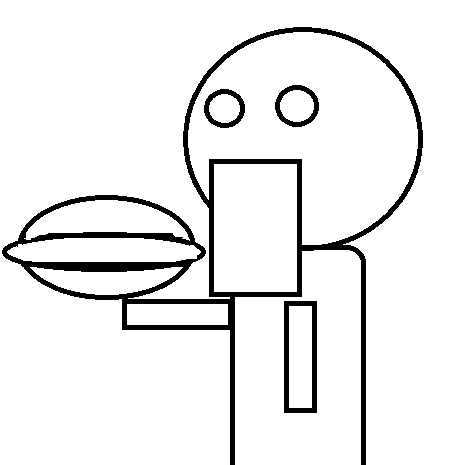
\includegraphics[width=5cm]{07lunch-music.png}
  \end{center}
\end{minipage}
%
\begin{minipage}{0.07\hsize}
  \quad
\end{minipage}



% - - - - - - - - - - - - - 

\end{document}
%
% お疲れさまです
%